\section{Corruption in the Absence of Concurrency Control}
\label{sec:db-corruption}

This section must be re-structured for ease of understanding.
First talk about transactions interleaving - narrative using fig 4.
Explain: Interleavings lead to half-corruption.
Exemplify half corruption using the first half of the code example.
Relate to dirty write..
Explain how half-corruption then leads to  sematic corruption and operational corruption.
Exemplify it using the second half of the coded example - unknown author.
Finally relate half corruption to Read Uncommitted.



\begin{figure}[htp]
  \centering
  \begin{subfigure}{\linewidth}
    \centering
    \begin{tikzpicture}[node distance=2cm]
  \node (v1) [big_vertex,xshift=0cm,yshift=0cm] {\small{\texttt{a:\textcolor{green}{Person}}}};

  \node (v2) [big_vertex,xshift=5cm,yshift=0cm] {\small{\texttt{b:\textcolor{green}{Book}}}};

  \node [below of=v1,yshift=1cm] {\small{\texttt{\textcolor{red}{name}:Tolkien}}};
  \node [below of=v2,yshift=1cm] {\small{\texttt{\textcolor{red}{title}:The Hobbit}}};

  \draw [thick,->,>=stealth] (0.8,0)  -- node [midway,above] {:\textcolor{green}{\small{\texttt{WROTE}}}} node [midway,below] {\small{\texttt{\textcolor{red}{year} = 1937}}} (2.4,0);
\end{tikzpicture}

    \caption{Logical view.}
    \label{hc-edge}
  \end{subfigure}
  %
  \begin{subfigure}{\linewidth}
    \vspace{2ex}
    \centering
        \begin{tikzpicture}[node distance=2cm,scale=0.6,every node/.style={transform shape}]

      \record(
      0,
      \small{\texttt{a:Person}},
      \small{\texttt{name:Tolkien}},
      $\boldsymbol{\rightarrow}$ \textbf{\small{\texttt{wrote b}}},
      \texttt{edge},
      \texttt{edge}
      );

      \record(
      -1,
      \small{\texttt{b:Book}},
      \texttt{property},
      \small{\texttt{title:The \hspace{-0.15cm} Hobbit}},
      ,
      \texttt{edge}
      );

      \record(-2,
      \small{\texttt{vertex id}},
      \texttt{property},
      \texttt{property},
      \texttt{edge},
      \texttt{edge}
      );


      \spaceRecord(-3)

      \record(-4,
      \small{\texttt{vertex id}},
      \texttt{property},
      \texttt{edge},
      \texttt{edge},
      \texttt{edge}
      );

    \end{tikzpicture}

    \caption{Storage view.}
    \label{hc-db-rep}
  \end{subfigure}%
  \caption{Logical and storage views of a reciprocally inconsistent edge \emph{ab}.}
  \label{hc}
\end{figure}

When a given transaction writes a distributed edge it must infact perform two writes, writing reciprocal entries in the adjacency lists at the source and the destination vertices, which say reside on servers $S_i$ and $S_j$ respectively. Without concurrency control, transaction's writes to a distributed edge can interleave producing a distributed edge in a \emph{half-corrupted} state - reciprocal consistency has been violated. Possible interleavings of concurrent writes to a distributed edge are given in Figure \ref{conf-scen}. A half-corrupted edge is an example of a \emph{dirty write} (ANSI \emph{P0} \cite{Berenson1995}, Adya \emph{G0} \cite{Adya2000}), which is proscribed by the weakest ANSI isolation level \textbf{Read Uncommitted}. Under Read Uncommitted the database ensures a total order on transactions, consistently ordering writes from concurrent transactions, which would prevent all interleavings in Figure \ref{conf-scen}.

For such half-corrupted edges there exists a correct and a incorrect entry. Note, the order in which the two writes take place is not constrained. For example, when updating an edge between \emph{a} and \emph{b} it is equally likely to update \emph{a} then \emph{b} as it is to update \emph{b} then \emph{a}. A graph with half-corrupted edges has suffered \emph{structural corruption}.

Now, if subsequent transactions read the incorrect entry of a half-corrupted edge and write further edges, \emph{semantic corruption} has been introduced into the database. Further semantic corruption spreads by the same mechanism. A database is said to be \emph{operationally corrupt} when a significant proportion of its data records are in a semantically corrupted state, rendering the database of little practical use. To illustrate the process of corruption, consider two transactions $T_x$ and $T_y$. $T_x$ deletes the \emph{wrote} edge and $T_y$ appends a property \emph{year}:
\begin{Verbatim}[commandchars=\\\{\},fontsize=\small,xleftmargin=.2in]
\textcolor{grey}{// Tx}
\textcolor{blue}{MATCH} (a:\textcolor{green}{Person})-[w:\textcolor{green}{WROTE}]->(b:\textcolor{green}{Book})
\textcolor{blue}{WHERE} a.\textcolor{red}{name} = 'Tolkien' \textcolor{blue}{AND} b.\textcolor{red}{title} = 'The Hobbit'
\textcolor{blue}{DELETE} w

\textcolor{grey}{// Ty}
\textcolor{blue}{MATCH} (a:\textcolor{green}{Person})-[w:\textcolor{green}{WROTE}]->(b:\textcolor{green}{Book})
\textcolor{blue}{WHERE} a.\textcolor{red}{name} = 'Tolkien' \textcolor{blue}{AND} b.\textcolor{red}{title} = 'The Hobbit'
\textcolor{blue}{SET} w.\textcolor{red}{year} = 1937
\end{Verbatim}
Any interleaving in Figure \ref{conf-scen} will result in the half-corrupted edge displayed in Figure \ref{half-corrupted}. Assume, the correct ordering of transactions is $T_y$ then $T_x$ and the edge between \emph{a} and \emph{b} should still exist. The following transaction, $T_z$, introduces semantic corruption if it starts at \emph{b} and adds a new \emph{wrote} edge to an ``unknown author'' vertex. Further corruption spreads by the same mechanism.

\begin{Verbatim}[commandchars=\\\{\},fontsize=\small,xleftmargin=.2in]
\textcolor{grey}{// Tz}
\textcolor{blue}{MATCH} (b:\textcolor{green}{Book}),(u:Person)
\textcolor{blue}{WHERE NOT} (:\textcolor{green}{Person})-[:\textcolor{green}{WROTE}]->(b:\textcolor{green}{Book})
\textcolor{blue}{AND} u.\textcolor{red}{name} = 'unknown'
\textcolor{blue}{CREATE} (u)-[:\textcolor{green}{WROTE}]->(b)
\end{Verbatim}
